\chapter{Steps to calculate crlog}
Before starting to implement $cr\log$, we will see what are its 
steps.\\
According to \cite{le2016computing}, first, we filter the special cases. Then, we
 reduce the argument range. After, we use the polynomial approximation and 
 evaluation.

\section{Special cases}
In the special cases, we have five possibilities:
\begin{itemize}
    \item input is $NaN$ return $NaN$
    \item Input is negatif return $NaN$
    \item Input is $+0$ or $-0$ return $-\infty$
    \item Input is $+\infty$ return $+\infty$
    \item Input is a \textbf{subnormal} number. We transform it into \textbf{normal} number then we calculate as if it is normal.
\end{itemize}

\section{Argument reduction}
We know that $\log(x.y) = \log(x) + \log(y)$. 
We have in $Input = 2^E \times m$ with $E$ is the \textbf{exposant} and $m$ is the \textbf{mantissa}.\\
So we have $\log(Input) = E \times \log(2) + \log(m)$. \\
First, we calculate $\log(m)$ with \textbf{Tang}'s algorithm and \textbf{Gal}'s algorithm.

%%%%%%%%% explanation of the algos used to reduce the argument %%%%%%%%
\subsection{ \textbf{Tang}'s Algorithm} \label{subsection:Tang}
With $x=m*2^e$ and so that $\log(x) = \log(m) +e*\log(2)$\\
First, we  calculate $\log(m)$ with \textbf{Tang}'s Algorithm (\cite{le2016computing}) .\\
We have  two possibilities: either we make a single reduction or two reductions with this algorithm.\\

\begin{figure}[H]
    \centering
    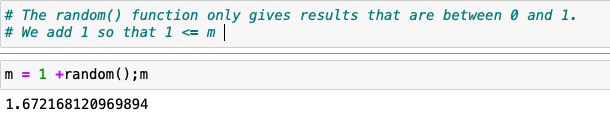
\includegraphics[width=\textwidth]{images/approche_de_Tang/Tang_intro.png}
    \caption{$m$ taken in random to test}
\end{figure}

\subsubsection{\textbf{Tang}'s algorithm with a single reduction}
We have :  $1 \le m < 2$ and we want to reduce $\log(m)$ using \textbf{Tang}'s algorithm.\\
First , we  use $k$ significant bits after the initial $1$. Then, we  take $i$ which represents the integer of the $k$ bits:\\
So we have:  $0 \le i < 2^k$ et $1+\frac{i}{2^k} \le m < 1 +\frac{i+1}{2^k}$\\
We look for $\alpha_i$ such as $1 \le m * \alpha_i < 1+\epsilon_i$ with $\epsilon_i$ as small as possible.
We can write $m = \frac{m * \alpha_i}{\alpha_i}$ and therefore have $\log(m) = \log(m * \alpha_i) - \log(\alpha_i)$.
After calculation, we have $\alpha_i = \frac{2^k}{2^k+i}$ and $\epsilon_i = \frac{1}{2^k+i}$ as $0 \le i < 2^k$ then the value $max(\epsilon_i) = \frac{1}{2^k}$.

If we take $m^{'} =  m * \alpha_i$, so we have $1 \le m^{'} < 1+\frac{1}{2^k}$. At the end of this algorithm,  $m^{'}$ has it's $k$ first zero bits after the initial $1$.

The value to be calculated has been reduced to $\log(m) = \log(m^{'}) - \log(\alpha_i)$ with $-\log(\alpha_i)$ which is already calculated and memorized in a table.\\

\begin{figure}[H]
    \centering
    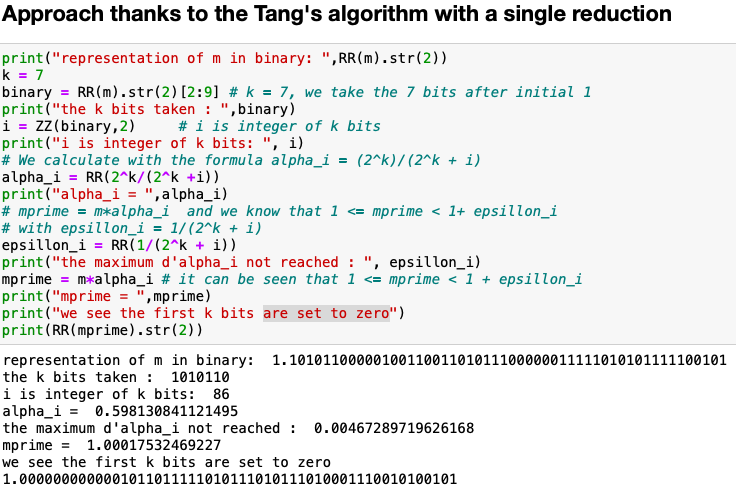
\includegraphics[width=\textwidth]{images/approche_de_Tang/Tang_1.png}
    \caption{The first reduction with $k = 7$}
\end{figure}


\subsubsection{\textbf{Tang}'s algorithm with two reductions}

After the first reduction explained above, another reduction is made again with the same value of $k$ for the following bits of the first reduction. Then, we  take $j$ which represents the integer of the $k$ bits. So we have : $0 \le j < 2^k$ and $1+\frac{j}{2^{2k}} \le m^{'} < 1 +\frac{j+1}{2^{2k}}$.

Now, we are looking for $\beta_j$ such as $1 \le m^{'} * \beta_j < 1+\epsilon^{'}_j$ with $\epsilon^{'}_j$ as small as possible. We have that $\log(m^{'})= \log(m^{'}*\beta_j) - \log(\beta_j)$.\\
After calculation : $\beta_j = \frac{2^{2k}}{2^{2k}+j}$ and $\epsilon^{'}_j = \frac{1}{2^{2k}+j}$. \\
As we have $m^{"} = m^{'}*\beta_j $ then $1 \le m{"} < 1 + \frac{1}{2^{2k}}$ .\\
So, we have $\log(m) = \log(m^{"}) - \log(\beta_j) - \log(\alpha_i)$.\\ 
$(-\log(\alpha_i))$  and  $(-\log(\beta_j))$ are already calculated and are put into memory in a table.
\begin{figure}[H]
    \centering
    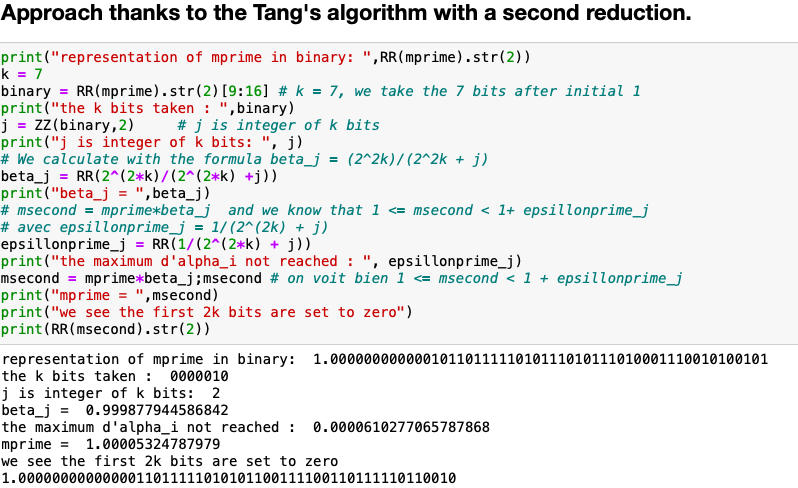
\includegraphics[width=\textwidth]{images/approche_de_Tang/Tang_2.png}
    \caption{The second reduction with $k = 7$}
\end{figure}

\subsection{\textbf{Gal}'s method with double precision}
\textbf{Gal}'s method is taken from \cite{gal1986computing}.\\
We have $x = y*2^n$ with $n$ integer and $0.75 \le y <1.5$\\ 
So  $\log(x) = \log(y)+n*\log(2)$.\\
We calculate $\log(y)$ using a table of triplets ($X_i$,\ $\log(X_i)$,\ $\frac{1}{X_i}$) with $0 \le i \le 192$.\\
$X_i = 0.75 + \frac{i}{256}+ \frac{1}{512} + E_i$ (with $E_i$ a very small number).\\
$\log(y) = \log(\frac{X_i*y}{X_i})  = \log(X_i)+\log(1+\frac{y-X_i}{X_i})= \log(X_i) + \log(1+z)$\\
If $X_i$ is choosen close to $y$, we have $\frac{-1}{384} < z < \frac{1}{384}$\\
and if more $y$ is close to 1 so $\frac{-1}{512} < z < \frac{1}{512}$.\\
We use an approximation polynomial $p(z)$ of degree $6$ (for double precision) to approach the function $\log(1+z)$.\\
If $x$ is close to $1$ so we use an approximation polynomial of $\log(x)$ without the table with a relative error of $2^{-72}$ which is negligible.\\
The table of the triplets ($X_i$, $\log(X_i)$, $\frac{1}{X_i}$) contains $576$ elements.\\
$F_i = \log(X_i)$ and $G_i = \frac{1}{X_i}$ with $0 \le i \le 192$.

The numbers $X_i$ are choosen so that $F_i$ and $G_i$ are $56$ bits of mantissa. And they have a relative precision of $2^{-65}$.\\
We search to be close to $0,75 +\frac{i}{256} + \frac{1}{512}$ with $X_i$ such that bits $57$ to $67$ of the mantissa of $\log(X_i$) and of $\frac{1}{Xi}$ which will be reset either all to $0$ or all to $1$. That's why small numbers $E_i$ were introduced. $F_i$ and $G_i$ are  the numbers with double precision obtained by a calculation of extended precisions and a symmetric rounding. 

\subsection{method with \textbf{Tang} algorithm and \textbf{Gal} method}
Our routine involves the two algorithms seen previously.\\
We start using \textbf{Tang}'s algorithm.\\
at the beginning as explained in \ref{subsection:Tang}, we only have $x=m*2^e$ and therefore we have $\log(x) = \log(m) +e*\log(2)$.\\
As mentioned in \ref{subsection:Tang}, we recover  $\alpha_i$ with the calculation:\\
$\alpha_i = \frac{2^k}{2^k+i}$ except for the following we will take $\alpha^{'}_i$ a double close to  $\alpha_i$ such that the $\log(\alpha^{'}_i)$ is the closest to a double .\\
This $\epsilon_i$ will be used to search for the $\log(\alpha^{'}_i)$ such that the bits from $54^{th}$ to $71^{st}$  are identical. (To have an approximation approximately  $2^{-71}$). (Figure \ref{fig:tang-gal})\\


\begin{figure}[H]
    \centering
    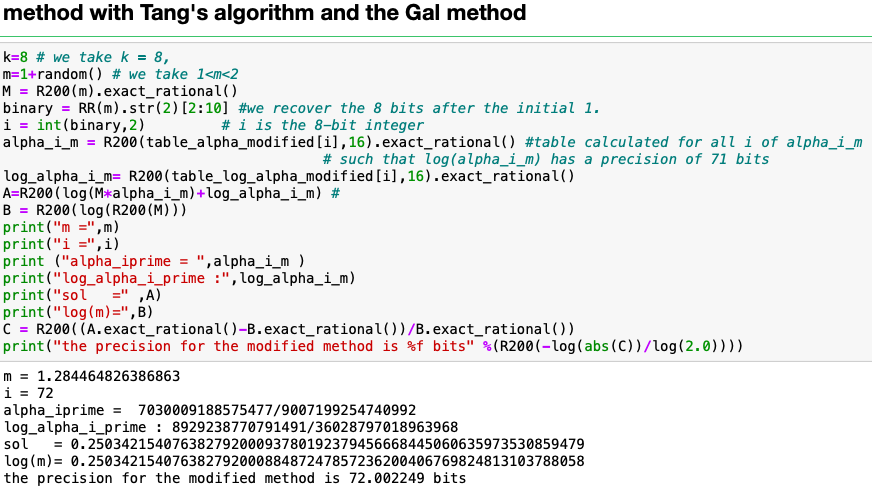
\includegraphics[scale = 0.49]{images/notre_met_Tang_Gal/algo_Tang_Gal.png}
    \caption{The revised method of \textbf{Tang} and \textbf{Gal}}\label{fig:tang-gal}
\end{figure}

We are going to verify if we obtain the same result with the \textbf{Tang} algorithm and our modified method (Figure \ref{fig:met_tang-gal}).
\begin{figure}[H]
    \centering
    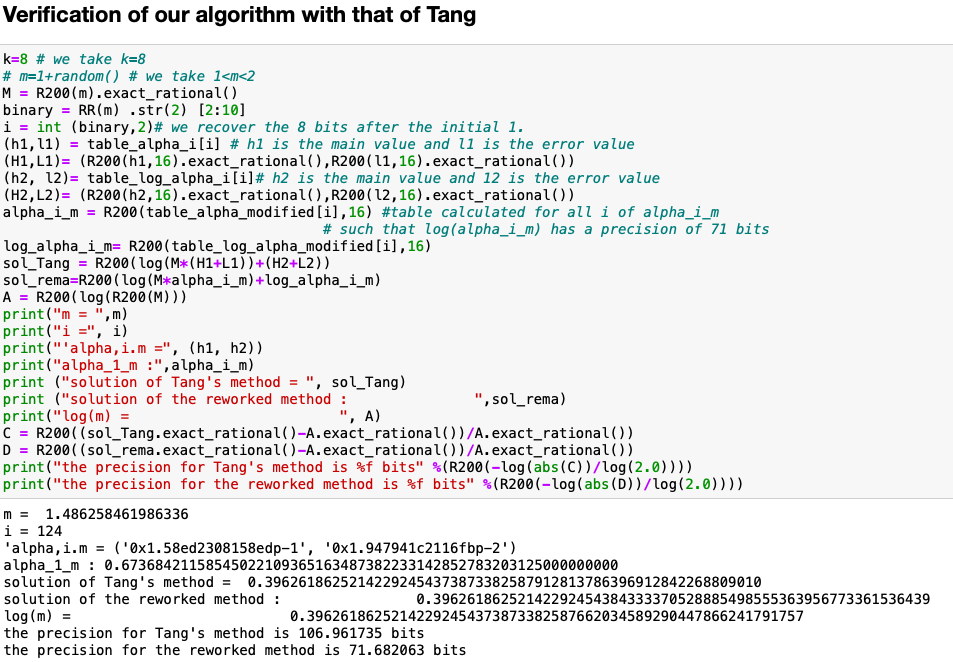
\includegraphics[scale = 0.46]{images/notre_met_Tang_Gal/algo_remanie.png}
    \caption{Verification of the revised method and \textbf{Tang}'s method}\label{fig:met_tang-gal}
\end{figure}

\section{polynomial approximation and evaluation}

Before calculating the approximation function with the \textbf{Sollya} tool, we will look for the interval for which the polynomial will be effective
for $m*\alpha^{'}_i$\\ with $0\le i<256$ and $1+\frac{i}{256}\le m < 1+\frac{i+1}{256}$ .
The calculations are experimented on \textbf{sage}, see the diagram \ref{fig:poly}:
\begin{figure}[H]
    \centering
    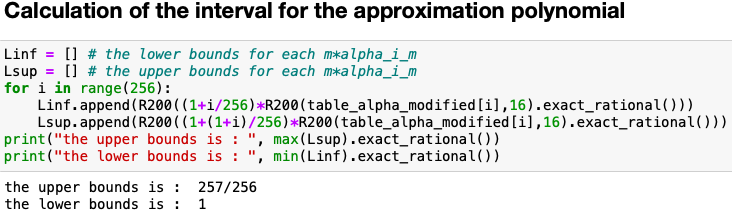
\includegraphics[scale = 0.49]{images/notre_met_Tang_Gal/calcul_intervalle.png}
    \caption{Interval calculation for the approximation polynomial }\label{fig:poly}
\end{figure}
We find as result $1 < m.\alpha^{'}_i < \frac{257}{256}$, exactly the same bounds as we calculated with the \textbf{Tang} method.\\
At the end of the calculation of the modified algorithm  from Tang and Gal's algorithm, we have that $\log(input) = \log(m.\alpha_i) - \log(\alpha_i) + E.\log( 2)$. We transform $ \log(m.\alpha_i)$ into $\log(1+t)$ to use the approximation function; then we have $t = m.\alpha_i-1$.\\
We search the polynomial approximation for $\log(1+t)$ thanks to the \textbf{Taylor} formula.\\ 
Let $P(t)$ the polynomial approximation for $\log(1+t)$, we have $P(t) \approx t - \frac{t^2}{2}...$, in case we have a constant term, we can reduce it to $0$.\\
This calculation  will be done thanks to the \textbf{Sollya} tool with its \textbf{fpminimax} function with the calculated interval.\\
Then we evaluate this approximation function with the argument $t = m.\alpha_i-1$.\\
Now, we have the operation $\log(input) = P(m.\alpha_i-1) - \log(\alpha_i )$(Figure \ref{fig:P}).\\

\begin{figure}[H]
    \centering
    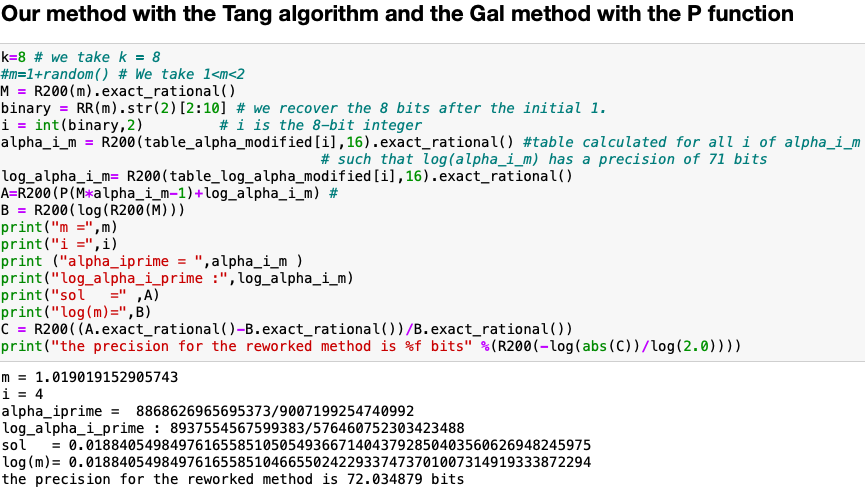
\includegraphics[scale = 0.49]{images/notre_met_Tang_Gal/algo_remanie_avec_P.png}
    \caption{The revised method  of \textbf{Tang} and \textbf{Gal} with $P(t)$}\label{fig:P}
\end{figure}

Before talking about the implementation of $cr_{\log}$, we will first see 
the used algorithms.\\

The algorithms of the chapter $4$ and chapter $5$ are taken from \cite{daramy2009cr} and \cite{lauter2005basic}.